\label{texfile:Installation}
\index{Installation}
The first step in the software installation process is to obtain the \mut\ examples, executables and database files from
\url{https://github.com/Grdbldr/MUT_Source.git}.  



\github\footnote{\url{https://github.com/} }. 


For the end user, who is \textbf{not interested in fortran programming or working with source code} you can skip to Section~\ref{section:allusers}.

\section{Software Developer}\label{section:softwareDev}
Source code and compiled executables for \mut\ and \mfu\ are available through   Through the \github\ website, you will need to e footnote at the bottom of this page
For the developer who \textbf{would like to modify and compile source code} we recommend that you obtain the following software development tools:
\begin{enumerate}
\item 
    \item Obtain the \mut\ source from the git repository at \url{https://github.com/Grdbldr/MUT_Source.git}.
    \item 
\end{enumerate}
For those unfamiliar with Git see for example the free software \github\ at \url{https://en.wikipedia.org/wiki/GitHub}.

\section{All Users}\label{section:allusers}


Before you run \mut\ for the first time, you need to define a windows environment variable called \bin.  An easy way to do this is to start a command prompt window from \textsc{File Explorer} by clicking an 
    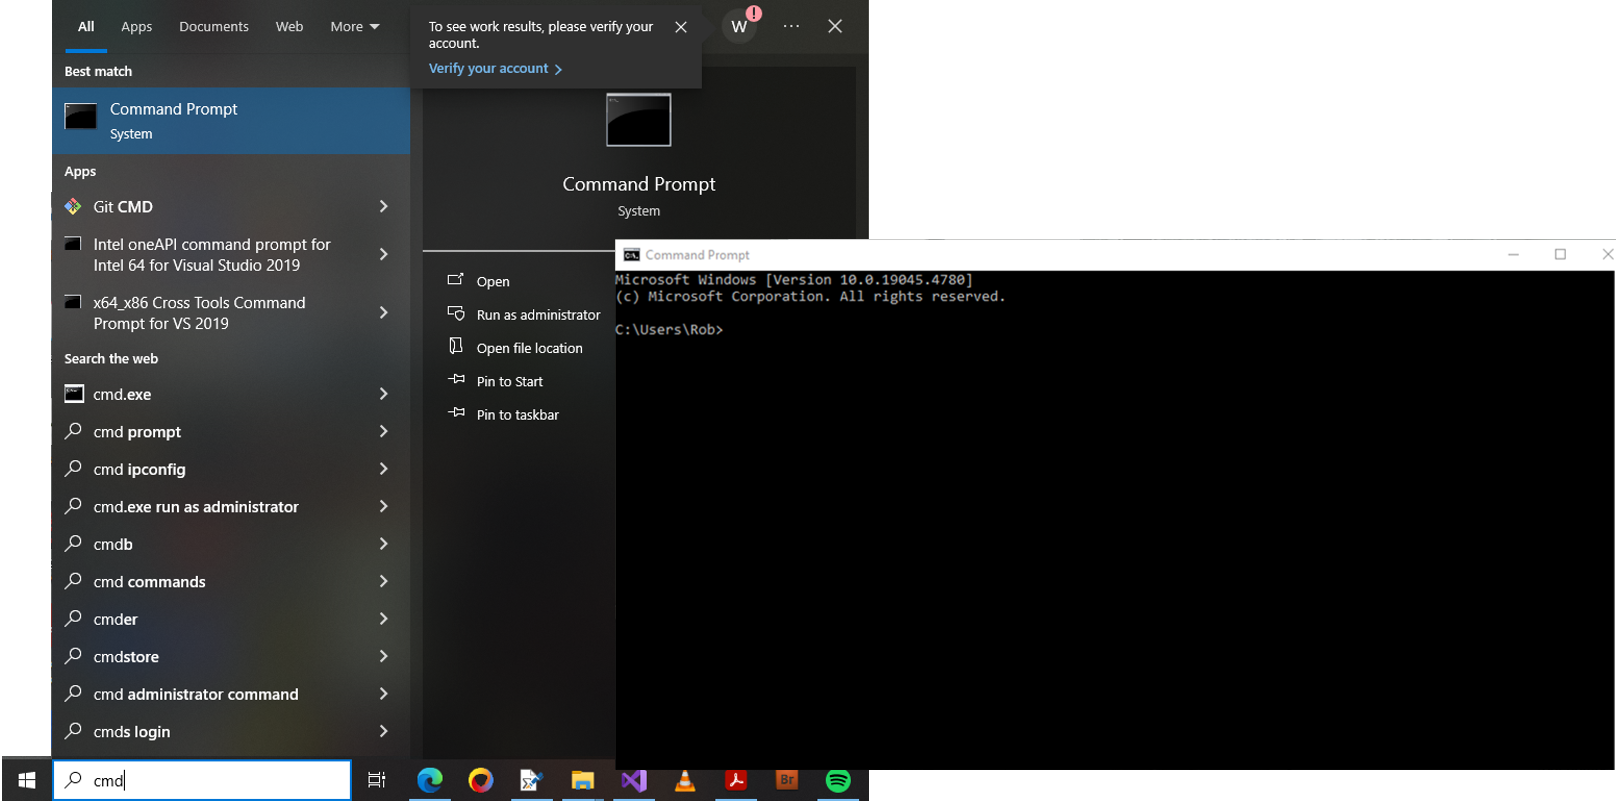
\includegraphics[width=0.8\textwidth]{commandPrompt_trimmed}

\begin{verbatim}
    set USERBIN=c:\bin
\end{verbatim}
This can be done through Windows settings or at the command prompt.

The software has been developed and tested under Windows 10 and \tecplot 360 EX 2018 R2.


    Build the source in Microsoft Visual Studio.  We provide a Visual Studio 2019 solution file for this purpose. Currently, Microsoft is providing a free community version of Visual Studio 2022.
